\documentclass{article}
\usepackage{xcolor}
\usepackage{verbatim}
\usepackage{fancyvrb}
\usepackage{colortbl}
\usepackage{caption}
\usepackage{subcaption}
\usepackage{multicol}
\usepackage{amsfonts}
\usepackage{mathtools}
\usepackage{changepage}
\usepackage{enumitem}
\usepackage{gensymb}
\usepackage{csquotes}
\usepackage{float}
\usepackage{listings}
\usepackage{amssymb}
\usepackage{amsthm}
\usepackage{amsmath}
\usepackage[hidelinks]{hyperref}
\usepackage[
	left=1in,
	right=1in,
	top=1in,
	bottom=1in
]{geometry}
\usepackage[utf8]{inputenc}
\usepackage{csquotes}
\usepackage{graphicx}
\usepackage[english]{babel}
\usepackage[
	backend=bibtex,
	style=authoryear,
	citestyle=authoryear
]{biblatex}
\addbibresource{~/.config/assets/LaTeX/auni.bib}

\setboolean{@twoside}{false}
\setlength{\parskip}{1em}
\setlength{\parindent}{4em}
\renewcommand{\baselinestretch}{1}
%\makeatletter
%\renewcommand{\@seccntformat}[1]{}
%\makeatother

\theoremstyle{definition}
\newtheorem{exmp}{Example}[section]
\definecolor{codegray}{rgb}{0.5,0.5,0.5}
\definecolor{backcolour}{rgb}{0.95,0.95,0.92}
\lstdefinestyle{mystyle}{
    backgroundcolor=\color{backcolour},
    basicstyle=\ttfamily\footnotesize,
    breakatwhitespace=false,
    breaklines=true,
    captionpos=b,
    keepspaces=true,
    showspaces=false,
    showstringspaces=false,
    showtabs=false,
    tabsize=2
}
\lstset{style=mystyle}

\author{Chris Sobczak}
\title{Survey of University Server Software}

\begin{document}
\begin{titlepage}
\maketitle

\vspace*{\fill}

\section{Abstract}
Universities, especially in the United States have consistently
increased the cost of attendance for their students with
no transparent cause. Some investigation and speculation
includes administrative costs, tenure, research expenses
and increasing security threats (\cite{ronald2009}).
A nominally large amount of money is spent on proprietary
software licenses for services like Microsoft Office 360,
SAS, SPSS and licenses for their own web services like
Microsoft Express, Red Hat Enterprise Linux, and other
server infrastructure.
The goal of the survey is to determine the market share
that open source server software occupies in the academic
setting.
The
figure to be estimated is the proportion of university web
services licenses. Are universities taking advantage of
the secure, free, and open source industry standard technologies
like nginx and Apache?
This study target population includes
all computers that
universities run for their websites, mail servers and other
digital services that provide a portal for students and
members of the public to access. The main focus of the study
is on those public domain services, and not services like
ftp servers and other internal affairs.

\end{titlepage}


\begin{flushleft}
\begin{multicols}{2}

\section{Background}
Open source software or ``free and open source software'' (FOSS)
is a piece or package of software
that is distributed with the source code available for
auditing and editing. The statistical software R is a
great example of a flourishing FOSS project where
users are able to contribute to the project and create new
packages. Another example is the OpenBSD operating system.
In the case of OpenBSD and other FOSS operating systems,
the public has the ability to know exactly what is going
on behind the scenes. This is not to say that every user
is required to read and understand the low level source
code, but it is a principle that the project is transparent
and the software community can audit it, creating a web of trust.

In contrast, there is no reason for a consumer to trust
in the word of a company that distributes closed source
software. This organization can claim whatever they want
about the security and privacy of their software but
without having the right to audit the source code,
there is no reason to believe any of those claims.
This raises security concerns in proprietary software since
if the only way a software package is considered \textit{secure}
is by the fact that no one knows how it works except the producer,
then as soon as the code becomes available (due to a leak), it can
all be considered compromised. This happens constantly with the Microsoft
Windows operating system, as we have seen most recently with the Solar
Winds attack (\cite{solarwinds2021}).
FOSS is secure through industry standard
security schemes, cryptography and by the knowledge of the thousands
of programmers who have access to it (compared to the relatively
smaller number of people who work on a single companies development
team).

Finally, maybe the more important reason for institutions,
FOSS is also (most of the time) free of cost (in addition
to ``free as in freedom'').
Universities and other public institutions
spend millions of dollars each year on software licenses
for their students, staff and web services and other
infrastructure. Increasing costs for post-secondary education and
healthcare administration costs can be attributed to some extent to
these rising software licensing prices and the constant
need for cybersecurity improvements. The increasing costs
make higher education less accessible and harm the most
vulnerable populations who rely on affordable healthcare.
A very obvious way to reduce
costs is be replacing these proprietary packages with equivalent
and more secure, free, and open source software (\cite{kenny2000}).

In addition to the problematic cost of closed source, proprietary
software, these costly, licensed software packages are most vulnerable
to security threats.
Security should be a high priority of all organizations but
especially at public institutions where all of the software that staff and
students interact with poses a threat to those individuals.
Providing one for profit company exclusive access to your staff and
students, in the age of surveillance capitalism is quite reckless
(\cite{karen2018}).

So this study, establishes a base-line estimate
of the proportion of free and open source servers being used by
universities around the world.
The questions that are answered include:
Are there specific countries whose universities
use more open source servers than others? What kinds of services
are associated with certain operating systems?

\section{Methods}
This survey was conducted using cluster sampling.
The primary sampling unit (psu) being the name
of an institution, and the primary unit of interest
being the associated domain(s). Each of the schools
highest level registered domain names are probed to
extract all their associated subdomains, defining the secondary
sampling units (ssus).
A census was then taken of these ssus
to determine the software run at each public domain name and
calculate the proportion of the school's services that
run open source software.

To provide an example, if Simon Fraser University (SFU)
was draw into our sample, the unit of interest would be
their registered domain name \texttt{sfu.ca}. Using the
tool \texttt{findomain}, all of the subdomains under
\texttt{sfu.ca} are collected into a file and probed to see if the service is up.
Some example subdomains are \texttt{mailgate.sfu.ca},
\texttt{imapnew.sfu.ca}, and \texttt{canvas.sfu.ca} for
the schools email services and canvas portal. This is
only a very short list of some of the possible subdomains.
It is common to have thousands of subdomains associated
to the same top name for each school. Finally, filtering out all of
the services that are not up, the header of the service is pulled
using \texttt{curl}, which includes information about the software
running at that address. The results are cleaned aggregated and proportions
of the resulting categories are tabulated.
Details on the tools I used in \autoref{sec:tools} \hyperref[sec:tools]{Tools}.

For example, pulling the server information from \texttt{mail.sfu.ca} for
SFU's mail service results in \texttt{Microsoft-IIS/10.0} as it is a
Microsoft Exchange mail server. All responses including this, \texttt{MS},
\texttt{Win64}, and other server names that are licensed with anything
except the \textit{GPL}, \textit{BSD}, \textit{MIT}, or \textit{Apache}
licenses are considered proprietary, whereas those responses with
the mentioned licenses are considered open source.

\subsection{Survey Design}

Using cluster
sampling, a simple random sample (SRS) is taken of all the schools in the sampling
frame (\cite{Hipo}). This sampling frame is an open source dataset
of most of the universities in the world. Inevitably
this list will have omitted some schools, but the set
contains 9693 schools which is slightly on the low
end of estimates, which may introduce bias in the
conclusions of this study.

\subsection{Sample Size Selection}
The goal of this study is
to estimate the proportion of university servers
running an open source operating system using a 95\% confidence
interval with a margin of error of 0.03.
Therefore, using
\cite{lohr2019},
``\dots surveys in which one of the main responses of interest
is a proportion, it is often easiest to use that response
in setting the sample size.
For large populations, $S^2 \approx p(1-p)$, which
attains its maximal value when $p=1/2$. So using
$n_0=1.96^2/(4e^2)$ will result in a 95\% CI with width at most
$2e$.''

$$
	n_0
	=
	\frac{
		z^2_{\alpha/2}S^2
	}{
		e^2
	}
	=
	\frac{
		1.96^2(\frac{1}{2})(1-\frac{1}{2})
	}{
		e^2
	}
	\approx
	1067
$$

No need to use the finite population correction adjustment
since the sample size
is reasonable compared to the population size and the full
dataset can be collected with a reasonable amount of resources.

\subsection{Taking the Sample}
With an appropriate sample size of $n=1067$,
using an R script to
draw the sample, the selected school domains
are saved in the \texttt{data.Rda} file found
in the GitHub repository, along with \texttt{sample.R},
used to draw the sample.
Within the sample, 1049 schools have only
one registered domain, 16 schools have two
registered domains and 2 have three
domains.

$$
	N=9693, \ n=1067, \ m_0\approx2539008
$$

The following 18 schools that were drawn in the sample
have more than one domain name registered:
Augusta University,
University of Manchester,
Universidad del País Vasco,
Chinju National University of Education,
Royal Holloway and Bedford New College,
Northeastern University,
University of the Pacific,
Kwangju University,
Kwangwoon University,
University of Massachusetts at Lowell,
St. Mary's University,
University of Essex,
Chonnam National University,
Hanshin University,
Savannah College of Art and Design,
University of Technology Sydney,
Universitat Pompeu Fabra, and
Kyungil University.

These 16 schools with two domains and 2 schools with three domains
accounts for the total 1087 ($1067 + (16 \textrm{ duplicates}) +
(2\times2 \textrm{ more duplicates}) = 1087$) domains in the
\texttt{domains} file of the GitHub repository. This file
contained a few duplicates and subdomains for the school,
so some of the domains were repeated and some were just included within
the schools \texttt{subdomains/} file, reducing it to 1081 files
in \texttt{subdomains/}.

All domains were separated onto their own line of the \texttt{probing/domains}
file and processed with \texttt{findomain}.
When extracting the subdomains, the \texttt{gen-subdomains}
script only processed 1079 domains, identifying an inconsistency.
Three of these domains that were not processed were \texttt{aloma.edu},
\texttt{student.uts.edu.au}, and \texttt{www.clcmn.edu}. In the case of
\texttt{aloma.edu}, this is just a typo in the sampling frame for the
Alamo Colleges' domain, which naturally is corrected to \texttt{alamo.edu}.
The next missing domain \texttt{student.uts.edu.au}, for the University
of Technology Sydney in Australia which is just a subdomain for their
website \texttt{uts.edu.au}, identified as a duplicate domain.
Finally, \texttt{www.clcmn.edu} for
Central Lakes College-Brainerd is another subdomain for their college
that was already extracted from \texttt{clcmn.edu}, another duplicated domain.

In the GitHub repository, the file \texttt{domains} is the audited file containing all
of the highest level domains for the sample that the full observational information could
be extracted. Domains omitted from this file were unreachable as mentioned in the discussion.
From this file, the domains belonging to the same school have been concatenated
so that results can be organized by psu before calculating proportions.


\section{Results}
The full results dataset of proportion of servers at
each psu is available on the GitHub as \texttt{proportions.csv}.
The proportion of each license status is represented in the columns,
in addition to the sum for the FOSS licenses to compare with the
non-FOSS proportion. After the proportion is measured in each of
the psus, the population estimate is calculated using the
ratio estimator
$$
	\hat{\bar{y}}_r
	=
	\frac{
		\sum_{i \in S} M_i\bar{y}_i
	}{
		\sum_{i \in S} M_i
	}
	=
$$
with a standard error of
$$
	\textrm{SE}(\hat{\bar{y}}_r)
	=
	\sqrt{
		\left(
			1 - \frac{n}{N}
		\right)
		\frac{1}{n\bar{M}^2}
		\frac{
			\sum_{i \in S}M_i^2\left(\bar{y}_i-\hat{\bar{y}}_r\right)^2
		}{
			n-1
		}
	}
$$
$$
=
$$

\subsection{Nonresponses}
It is possible that the nonresponses are missing completely at random,
but it is more likely that the nonresponses are missing at random, given
covariates (\cite{lohr2019}). This is more likely since it is possible that
the unreachable schools and domains are correlated with other factors especially
the location of the school (country). Figure \ref{fig:props} in \autoref{sec:plots}
\hyperref[sec:plots]{Nonresponse per Country}
of the Appendix shows that the countries with the largest missing proportions
of schools are those that are furthest from the location the study was conducted.
It is also possible but less likely that
the nonresponse is correlated with the actual license of software used (the
response variable in this study), so we will be adjusting according to
the ``Missing at Random" scheme in \cite{lohr2019}. Figure \ref{fig:country}
validates this assumption, the countries with the highest proportions of
FOSS software are generally of the East, with a mix down the list.

In order to compensate for the nonresponse schools
in the sample, estimates are adjusted using weighting
class adjustment using countries as auxiliary variables. Table
\ref{table:weights} shows the
sum of weights, sample size, and respondents for each class
(\autoref{sec:weights} \hyperref[sec:weights]{Weighting Classes} of
the Appendix).
Only countries with nonresponses in the class are show.
Those not included in the picture maintain the same $N/n$ weighting.

For each of the countries of the table, $\hat{\phi}_c$ is defined as
$$
\hat{\phi}_c
=
\frac{
\textrm{sum of weights of respondents in class $c$}
}{
\textrm{sum of weights of a full sample in class $c$}
}
$$
With $c$ being the country, when the full sample was successfully returned,
$\hat{\phi}_c=1$, causing no impact on the calculated estimates for that country.
The weight factor is then the reciprocal of $\hat{\phi}_c$, $\frac{1}{\hat{\phi}_c}$.
The weight factor for countries not shown in Table \ref{table:weights} is $N/n$.
The new weights are calculated with
$$
\tilde{w}_i
=
w_i
\sum_{c}
\frac{x_{ci}}{\hat{\phi}_c}
$$
Let $x_{ci}=1$ if unit $i$ is in class $c$, and $0$ otherwise, so that
the new weights are adjusted according to their class specific $\hat{\phi}_c$.
Our estimate is then calculated using the estimator $\hat{\bar{y}}_{wc}$,
defined as
$$
\hat{\bar{y}}_{wc}
=
\frac{
	\sum_{i \in S} \tilde{w}_iy_i
}{
	\sum_{i \in S} \tilde{w}_i
}
=
$$

The weighting class adjustment estimator reduces the proportion of FOSS software
in use, suggesting that those countries that were less reachable showed an even
lower proportion of FOSS software.
This estimate for the proportions of licenses, although a slim majority, it is still
surprisingly
low. Considering the benefits of open source software, you would expect a
university to use proprietary software only when the specific legacy software
that they need to run can \textit{only} be run on a proprietary platform.

Despite that, we see that a big proportion of universities prefer paying for the
enterprise licenses and security risks, over free and secure alternatives. It shows
that within academic institutions, there is room to change and save money by
replacing the expensive software with free alternatives.

\subsection{Discussion and Conclusion}
Overall, the data supports the claim of the paper, that universities,
like other public institutions have room to improve and save money on
software and make better security choices.
The goal of this study is to hopefully shed
light on an opportunity for public institutions to improve their own
services and operation through choice of software. The most common
proprietary software found in the study is the Microsoft Express
server, the Windows email server distribution, like the one run at
\texttt{mail.sfu.ca}. Some FOSS alternatives to this include
\href{https://www.citadel.org/}{citadel},
\href{https://kolab.org/}{kolabcommunity}, and
\href{https://www.open-xchange.com/}{Open-Xchange}.

There are plenty more alternative schemes for running an email server like
these, that could replace Express, it is just a matter of
the information technicians of the school making the right software
decisions. That is what it comes down to the most, \textit{knowing}
there is even a decision to make. The technology industry giants have
such a strangle hold on the market and use malicious, anticompetitive
practices that cause consumers and businesses to think that they have
no choice except to pay for proprietary licenses (\cite{win2015}).

\subsection{Bias}
Although the sample size for the study is very large, some bias in the sample
could contribute to errors in the conclusions. One possible source of bias
is the sampling frame potentially not including \textit{all} universities in
the world. Inevitably, this is the case, however it seems reasonable to consider
the sample draw from the frame is representative of the target population
(244 schools from the US, 23 from Canada, 10 from Italy, and so on).

Another potential source of bias in this study includes a few technical
limitations. First, the \texttt{findomain} tool relies on databases and
other historical DNS records and methods to identify subdomains, but it
could miss some, most likely missing newly registered subdomains which
may not represent the true makeup of the schools services. Additional
bias could be introduced with \texttt{curl}, when it is not able
to make a connection, or the header of the document not included the required
server information for this study, the response is counted as an \texttt{NA}.
However, it is almost always the case, that these
missed, and unidentified servers are internal services, observational units that
are outside the scope of the target population, not considered in this study.

Finally, a few of the schools in the sample were unreachable for probing
The most common reason for the nonresponse was the absence of a
legitimate SSL certificate at any of the given domains or subdomains
preventing the data from being collected with curl
(\cite{curlSSL}).



\end{multicols}
\end{flushleft}
\printbibliography
\section{Appendix}

\subsection{Tools} \label{sec:tools}
The study was conducted using a combination of R, and shell scripting.
Whenever possible, the basic GNU utilities are preferred over more complex
ones, as well as the scripting style being POSIX compliant instead of Bash
specific. The following tools are those tools greater than the GNU basic utilities
that were used for the study.
All project source files can be found at this
\href{https://github.com/chrissobczak/os-survey}{GitHub} repository.

\subsubsection{Extracting All SSUs From Each PSU}
The tool \texttt{findomain} was used to collect all subdomains associated with a school.
A simple \texttt{findomain -t \$domain} can be run to collect a full set of the subdomains
for the given \texttt{\$domain}. However, as discussed, there may be limitations to any tool
attempting to collect all of these associated subdomains.
The R script outputs the base second and third level subdomains
into a file with one domain per line, for which I run \texttt{findomain -t}.
The tool takes a domain and searches various databases and tests the domain
for subdomains associated with it. I take this and output all the subdomains
into a file for each school, and then test if the service is up.

\subsubsection{Probing Hosts}
In order to save time in the data collection phase, I first validated the output
given from \texttt{findomain} by probing each provided domain with the
DNS lookup utility \texttt{dig}. This tool checks a DNS server to see if the
given domain actually exists and if the host is up. Without this step,
probing from each of the SSUs would take much longer.

\subsubsection{Extracting Info From SSUs}
The \texttt{probe-knownhosts} scripts are shell scrips
that run the following curl command on each line of each
psu file, collecting the server data.
\begin{lstlisting}
curl -I -s --connect-timeout 2 $domain
\end{lstlisting}
This outputs the header of the page that might look like the following from \texttt{mail.sfu.ca}:
\begin{lstlisting}
HTTP/1.1 302 Moved Temporarily
Cache-Control: no-cache
Pragma: no-cache
Content-Length: 0
Location: https://mail.sfu.ca/owa/
Server: Microsoft-IIS/10.0
X-FEServer: ITS-EXCHANGE06
X-RequestId: 66b65c01-b923-40f8-8337-ef6018996422
Date: Sun, 18 Apr 2021 06:1:45 GMT
\end{lstlisting}
The \texttt{Server} lines are extracted with \texttt{grep} and added to the results file for that school.

\subsubsection{Network Mapper}
At the beginning of the study, it was considered using the network mapping tool \texttt{nmap}.
There are several legal controversies surrounding the use of this tool since it probes all ports at
a given location and attempts to make connections. The advantage of this tool is greater identification
of operating system and other services at each location, however at the much greater cost of time and
risk.


\subsection{Weighting Classes} \label{sec:weights}
% latex table generated in R 4.0.5 by xtable 1.8-4 package
% Sun Apr 18 02:18:16 2021
\begin{table}[H]
\centering
\caption{Weighting Class Adjustment Factors}
\begin{tabular}{l|cccccc}
Country & \shortstack{Sample \\ Size} & Responses & \shortstack{Sum of \\ Sample Weights} & \shortstack{Sum of \\ Respondent Weights} & $\hat{\phi}_c$ & \shortstack{Weight \\ factor} \\
  \hline
Afghanistan &   4 &   3 & 36.33 & 27.25 & 0.75 & 1.33 \\
Argentina &  15 &  14 & 136.26 & 127.17 & 0.93 & 1.07 \\
Belarus &   5 &   4 & 45.42 & 36.33 & 0.80 & 1.25 \\
Belgium &   6 &   5 & 54.50 & 45.42 & 0.83 & 1.20 \\
Brazil &  22 &  20 & 199.84 & 181.67 & 0.91 & 1.10 \\
Canada &  23 &  22 & 208.93 & 199.84 & 0.96 & 1.05 \\
China &  44 &  39 & 399.68 & 354.27 & 0.89 & 1.13 \\
Colombia &  13 &   8 & 118.09 & 72.67 & 0.62 & 1.62 \\
Ecuador &   3 &   2 & 27.25 & 18.17 & 0.67 & 1.50 \\
Ethiopia &   4 &   3 & 36.33 & 27.25 & 0.75 & 1.33 \\
France &  30 &  25 & 272.51 & 227.09 & 0.83 & 1.20 \\
India &  44 &  35 & 399.68 & 317.93 & 0.80 & 1.26 \\
Indonesia &  16 &  12 & 145.34 & 109.00 & 0.75 & 1.33 \\
Iran &  21 &  17 & 190.76 & 154.42 & 0.81 & 1.24 \\
Iraq &   7 &   6 & 63.59 & 54.50 & 0.86 & 1.17 \\
Italy &  10 &   9 & 90.84 & 81.75 & 0.90 & 1.11 \\
Japan &  63 &  56 & 572.28 & 508.69 & 0.89 & 1.12 \\
Korea  &  29 &  26 & 263.43 & 236.18 & 0.90 & 1.12 \\
Latvia &   3 &   2 & 27.25 & 18.17 & 0.67 & 1.50 \\
Lebanon &   3 &   2 & 27.25 & 18.17 & 0.67 & 1.50 \\
Malaysia &  18 &  16 & 163.51 & 145.34 & 0.89 & 1.12 \\
Mongolia &   3 &   2 & 27.25 & 18.17 & 0.67 & 1.50 \\
Nigeria &  10 &   8 & 90.84 & 72.67 & 0.80 & 1.25 \\
Panama &   4 &   2 & 36.33 & 18.17 & 0.50 & 2.00 \\
Philippines &  13 &  10 & 118.09 & 90.84 & 0.77 & 1.30 \\
Poland &  11 &  10 & 99.92 & 90.84 & 0.91 & 1.10 \\
Puerto Rico &   3 &   2 & 27.25 & 18.17 & 0.67 & 1.50 \\
Russia &  26 &  23 & 236.18 & 208.93 & 0.88 & 1.13 \\
Rwanda &   2 &   1 & 18.17 & 9.08 & 0.50 & 2.00 \\
Saudi Arabia &   8 &   7 & 72.67 & 63.59 & 0.88 & 1.14 \\
Spain &   8 &   7 & 72.67 & 63.59 & 0.88 & 1.14 \\
Sudan &   8 &   4 & 72.67 & 36.33 & 0.50 & 2.00 \\
Syria &   4 &   3 & 36.33 & 27.25 & 0.75 & 1.33 \\
Taiwan &  10 &   7 & 90.84 & 63.59 & 0.70 & 1.43 \\
Tunisia &   2 &   1 & 18.17 & 9.08 & 0.50 & 2.00 \\
Turkey &  27 &  25 & 245.26 & 227.09 & 0.93 & 1.08 \\
Uganda &   4 &   3 & 36.33 & 27.25 & 0.75 & 1.33 \\
Ukraine &   9 &   8 & 81.75 & 72.67 & 0.89 & 1.12 \\
United Kingdom &  18 &  16 & 163.51 & 145.34 & 0.89 & 1.12 \\
United States & 244 & 222 & 2216.43 & 2016.59 & 0.91 & 1.10 \\
Uzbekistan &   4 &   3 & 36.33 & 27.25 & 0.75 & 1.33 \\
Venezuela &   4 &   3 & 36.33 & 27.25 & 0.75 & 1.33 \\
\end{tabular}
\label{table:weights}
\end{table}

\subsection{Nonresponses per Country} \label{sec:plots}
\begin{figure}[H]
\centering
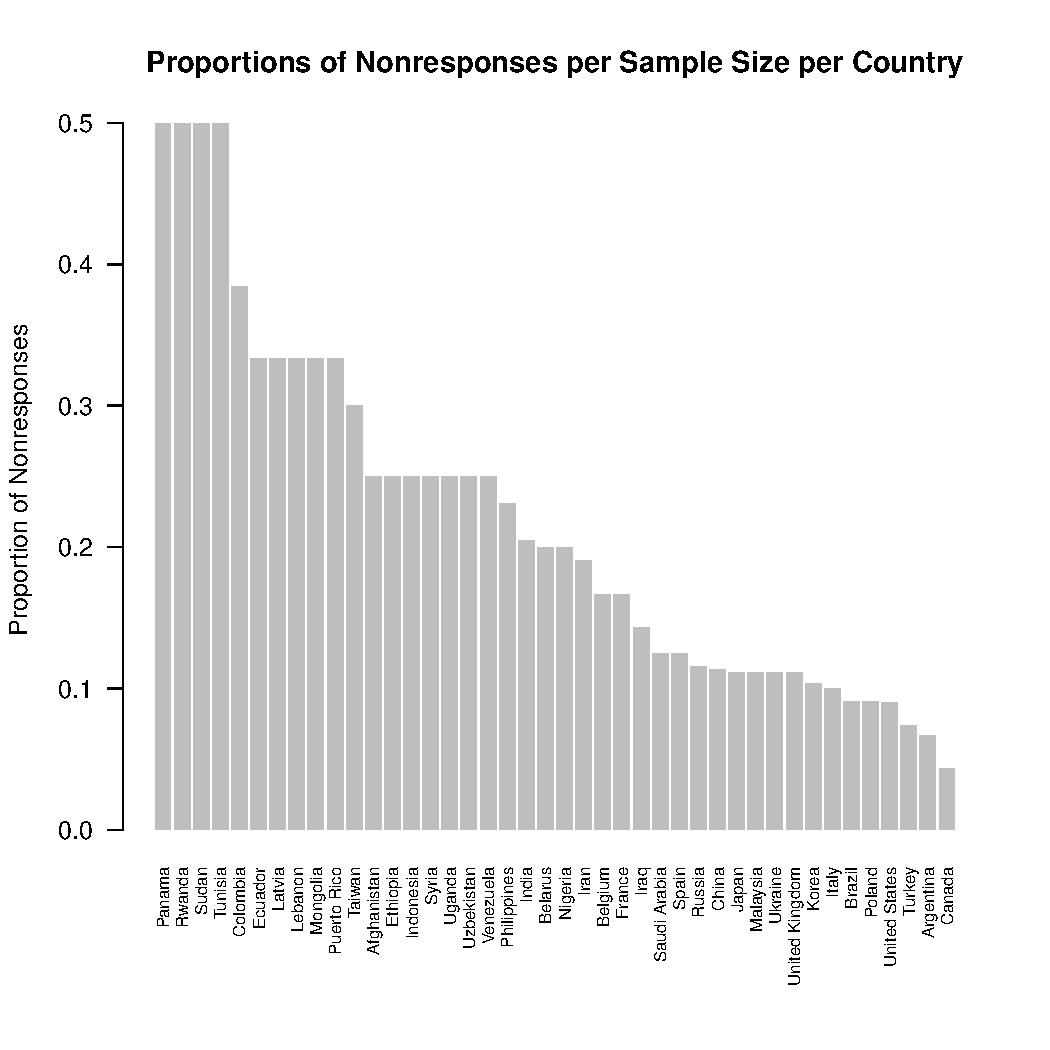
\includegraphics{graphics/missingprops.pdf}
\caption{Proportion of sample that is missed from the results as nonresponse}
\label{fig:props}
\end{figure}

\begin{figure}[H]
\centering
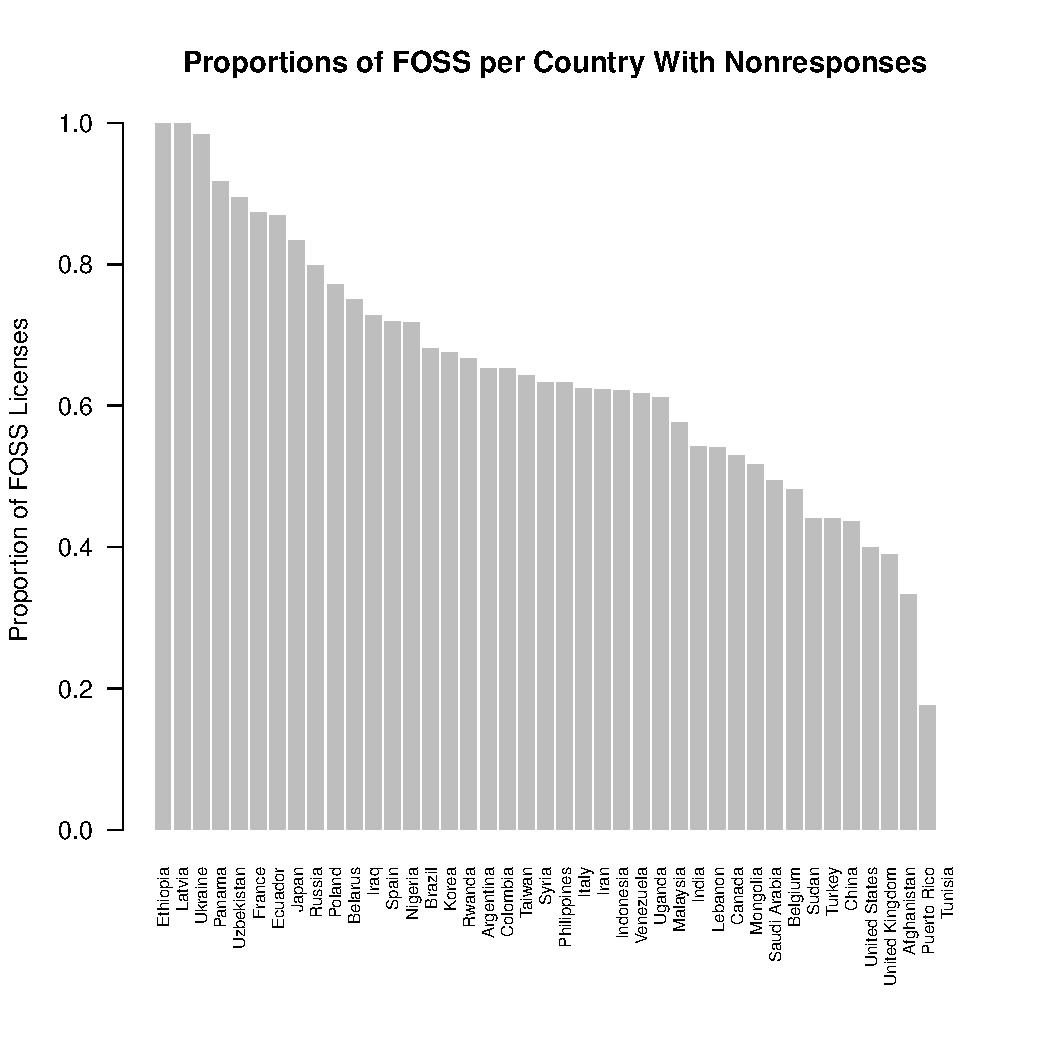
\includegraphics{graphics/country_props.pdf}
\caption{Of countries with nonresponses, the proportion of responses that are FOSS}
\label{fig:country}
\end{figure}

\end{document}
